	\documentclass[10pt,oneside]{CBFT_book}
	% Algunos paquetes
	\usepackage{amssymb}
	\usepackage{amsmath}
	\usepackage{graphicx}
% 	\usepackage{libertine}
% 	\usepackage[bold-style=TeX]{unicode-math}
	\usepackage{lipsum}

	\usepackage{natbib}
	\setcitestyle{square}

	\usepackage{polyglossia}
	\setdefaultlanguage{spanish}


	\usepackage{CBFT.estilo} % Cargo la hoja de estilo

	% Tipografías
	% \setromanfont[Mapping=tex-text]{Linux Libertine O}
	% \setsansfont[Mapping=tex-text]{DejaVu Sans}
	% \setmonofont[Mapping=tex-text]{DejaVu Sans Mono}

	%===================================================================
	%	DOCUMENTO PROPIAMENTE DICHO
	%===================================================================

\begin{document}

% =================================================================================================
\chapter{Método de separación de variables}
% =================================================================================================

Al resolver una PDE (partial differential equation) se termina en general en un problema de
Sturm-Liouville, que lleva a autovalores y autofunciones.

Un problema regular de Sturm-Liouville está representado por una ecuación del tipo
\[
	\dtot{}{x}\left[ r(x) \dtot{f}{x} \right] + [ q(x) + \lambda p(x)] f = 0,
\]
donde $p(x)$ es una función peso que definenla ortogonalidad (muchas veces vale 1).
Las condiciones de contorno en el intervalo $(a,b)$ serán
\[	
	f(a) + \dtot{f}{x}(a) = \qquad \qquad f(b) + \dtot{f}{x}(b) =
\]

En el (a,b) las condiciones de ortogonalidad se leen
\[
	\int_a^b \: U_n^*(\xi) U_m(\xi) p(\xi) d\xi = 0 \qquad n \neq m
\]
Asimismo, si están normalizadas, se puede escribir
\[
	\int_a^b \: U_n^*(\xi) U_m(\xi) p(\xi) d\xi = \delta_{nm}
\]
Luego, cualquier $f$ (well behaved) en el $(a,b)$ se puede poner como
\[
	f(x) \equiv \sum_{n=1}^N a_n U_n(x)
\]
Entonces
\[
	M_N = \int_a^b \: \left| f(x) - \sum_{n=1}^N \: U_n(x') \right|^2 \: dx,
\]
y esta expresión es mínima cuando los $a_n$ son
\[
	a_n = \int_a^b \: U_n^*(x') \: f(x') \: p(x') \: dx'
\]

Entonces,
\[
	f(x) = \sum_{n=1}^\infty \: U_n(x')
\]
es correcto porque la serie converge. Luego, integrando en $x'$
\[
	f(x) = \int_a^b \left[ \sum_{n=1}^\infty \: U_n^*(x') \: f(x') \: p(x') \: dx' \right] U_n(x)
\]
y donde
\[
	f(x) = \int_a^b \left[ \sum_{n=1}^\infty \: U_n^*(x') U_n(x) \right] \: f(x') \: p(x') \: dx'
\]
es claro que esto debe tener comportamiento de delta de Dirac, y
\[
	\sum_{n=1}^\infty \: U_n^*(x') U_n(x) = \delta(\vbx-\vbx')
\]
es la llamada condición de clausura.

% =================================================================================================
\section{Separación en coordenadas cartesianas}
% =================================================================================================

Separamos los problemas en regiones donde vale $\lapm{\phi} = 0$ entonces las fronteras tendrán la
$\rho(\vb{x}')$ en general en forma de $\sigma,\lambda$.

Para coordenadas cartesianas la ecuación de Laplace $\lapm{\phi} = 0$, adquiere la forma
\[
	\dpar[2]{\phi}{x} + \dpar[2]{\phi}{y}  + \dpar[2]{\phi}{z}  = 0,
\]
que intentaremos resolver a partir de un {\it ansatz} 
\[
	\phi(x,y,z) = X(x) \: Y(y) \: Z(z)
\]
lo que conduce a 
\[
	\frac{1}{X}\dtot[2]{X}{x} + \frac{1}{Y}\dtot[2]{Y}{y} + \frac{1}{Z}\dtot[2]{Z}{z} = 0.
\]
Para que esta solución valga, cada término tiene que ser una constante, entonces primeramente
\[
	\frac{1}{X} \dtot[2]{X}{x} = - \alpha^2
\]
lleva a 
\[
	\frac{1}{Y}\dtot[2]{Y}{y} + \frac{1}{Z}\dtot[2]{Z}{z} = \alpha^2,
\]
y 
\[
	\frac{1}{Y} \dtot[2]{Y}{y} = - \beta^2,
\]
conduce a
\[
	\frac{1}{Z}\dtot[2]{Z}{z} = \alpha^2 + \beta^2 = \gamma^2
\]
donde cada una de estas ecuaciones es una versión simplificada de Sturm-Liouville. En estos
casos particulares son osciladores armónicos; uno en cada dirección.
Luego suponiendo $\alpha,\beta \int \mathbb{R}>0$ será $\gamma \in \mathbb{R}$ y la solución 
general es
\[
	\phi(x,y,z) = \sum_{m=0}^\infty \sum_{n=0}^\infty A_{m,n} \euler^{\pm i\alpha_m x}
	\euler^{\pm i\beta_n y} \euler^{\pm i\sqrt{\alpha_m^2 + \beta_n^2 }z}.
\]
donde $A_{m,n}$ es una constante general. 
Las condiciones de contorno permitirán fijar las constantes y entonces la solución tendrá
diversas formas. 

Según la conveniencia del problema particular será
\[
	\euler^{\pm \gamma x_i } = \cosh( \gamma x_i ) + \sinh( \gamma x_i )
\]
\[
	\euler^{\pm i k x_i } = \cos( k x_i ) + i \sin( k x_i )
\]

\subsubsection{Algunos tips}

Queremos resolver la ecuación de Poisson, 
en el caso de cargas tipo (puntuales, lineales y superficiales)

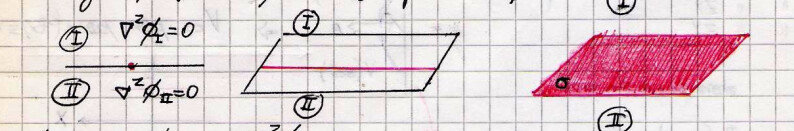
\includegraphics[width=0.4\textwidth]{images/fig_ft1_tips_separacion.jpg}

podemos resolver $\nabla^2 \vp = 0$ que es más sencilla y separamos en dos
regiones \textcircled{I} y \textcircled{II} donde me preocupo solamente
por Laplace.
Si las fuentes son más complejas que esto nos remitiremos a la función
de Green.

\begin{ejemplo}{\bf Potencial en una caja}

En este caso interesa el potencial $V$ dentro de la caja. El exterior está fuera del ámbito
de la resolución.

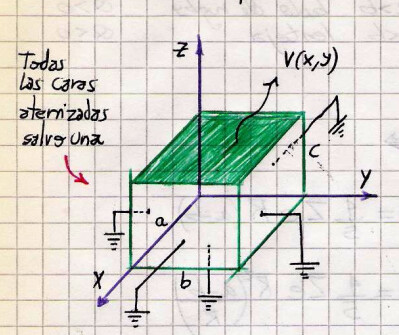
\includegraphics[width=0.4\textwidth]{images/fig_ft1_potencial_caja.jpg}

Se plantea para el potencial 
\begin{multline*}
	\phi(x,y,z) =  \sum_{\alpha,\beta} \:
	\left[ A_\alpha\sin( \alpha x) + B_\alpha\cos( \alpha x) \right]
	\left[ C_\beta\sin( \beta y) + D_\beta\cos( \beta y) \right]\times \\
	\left[ E_\gamma\sinh( \gamma z) + F_\gamma\cosh( \gamma z) \right]
\end{multline*}
Utilizando que el potencial es nulo en los contornos indicados (ver figura) resulta
\[
	\phi(0,0,0) = 0 \qquad \longrightarrow \qquad F_\gamma = 0
\]
\[
	B_\alpha = 0 \qquad D_\beta = 0
\]
\notamargen{Tal vez poner que esto es por las tapas laterales.}

Entonces, juntando todas las constantes en una única constante $A$ el potencial será la 
suma siguiente
\[
	\phi(x,y,z) =  \sum_{\alpha,\beta} \:
	A_{\alpha\beta} \: \sin( \alpha x) \: \sin( \beta y) \: \sinh( \gamma z)
\]
donde dada la relación $\gamma^2 = \alpha^2 + \beta^2$ este índice se ha absorbido junto a los
otros dos de manera que solo es una doble sumatoria.

Para satisfacer las condiciones de potencial nulo en $x=a$ y en $y=b$ se deben cumplir
\[
	\alpha = n \frac{\pi}{a} \qquad \beta = m \frac{\pi}{b}
\]
para todo natural $n, m$. Luego
\[
	\gamma = \pi \sqrt{ \frac{n^2}{a^2} + \frac{m^2}{b^2} }.
\]
Entonces, cambiando los índices de la sumatoria a
\[
	\phi(x,y,z) =  \sum_{n,m} \:
	A_{nm} \: \sin\left( n \frac{\pi}{a} x \right) \: \sin\left( m \frac{\pi}{b} y \right)
	\: \sinh\left( \pi \sqrt{ \frac{n^2}{a^2} + \frac{m^2}{b^2} } z \right)
\]

Finalmente sobre la tapa superior será $\phi(x,y,c) = V(x,y)$ de manera que, mediante un
cálculo rutinario llegamos a
\[
	A_{nm} = \frac{4}{ a b \sinh( \pi \sqrt{ n^2/a^2 + m^2/b^2} c )} \:
	\int_0^a \int_0^b \: V( x,y) \: \sin\left( n \frac{\pi}{a} x \right) \: 
	\sin\left( m \frac{\pi}{b} y \right) \: dy dx.
\]

\end{ejemplo}

\begin{ejemplo}{\bf Problema 2}

El problema a resolver está en el sketch de abajo

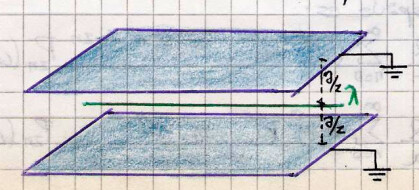
\includegraphics[width=0.4\textwidth]{images/fig_ft1_problema2_sep_A.jpg}

Queremos que no haya carga en las regiones en las cuales se subdividiráel
espacio nos ocuparemos del laplaciano.

El sistema coordenado a utilizar está mostrado abajo

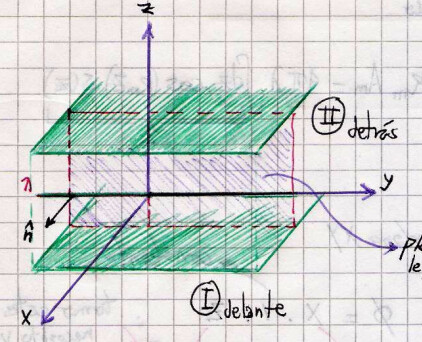
\includegraphics[width=0.4\textwidth]{images/fig_ft1_problema2_sep_B.jpg}

La densidad de carga se puede escribir según
\[
	\rho(\vbx) = \lambda \delta(x) \delta(z) = \sigma \delta(z)
\]
donde hemos definido una densidad $\sigma$.
La solución será de la forma
\[
	\Phi = X \: Y \: Z,
\]
donde $Y$ será una constante porque el problema no depende de $y$.
Como las funciones trigonométricas se anulan en puntos y $Z$ necesita
esto se eligen
\[
	Z \propto \cos( k_z z ), \sin( k_z z )
\]
y $X \propto \euler^{- K x} $ porque el potencial podría ir decreciendo
en $x$ --aunque es infinito--.
Donde $K=k_z$ y $k_y=0$. Hay una simetría en $xy$ de reflexión, entonces el
potencial es par. Luego, para la base de funciones usaré funciones pares
(cosenos).
Luego,
\[
	\phi(z=\pm a/2) = 0,
\]
por ser planos conductores a tierra. Entonces hacer que se cumpla
\[
	\cos(\pm a/2 K) = 0,
\]
necesita $k_n = ( 2n + 1 ) \pi / a$ (nos alcanza con $\mathbb{N}$ más el cero).
La base de funciones será
\[
	\phi_I = \sum \: A_n^I \: \euler^{-K_n x} \: \cos(K_n z) \qquad 
	x > 0
\]
\[
	\phi_{II} = \sum \: A_n^{II} \: \euler^{K_n x} \: \cos(K_n z) \qquad 
	x < 0
\]

Ahora pediremos condiciones en la superficie de seperación, la continuidad
del potencial
\[
	\phi_I( x=0 ) = \phi_{II}( x=0 )
\]
Entonces, para el campo resultan
\[
	\sum_n^\infty A_n^{I} \cos(k_nz) = 
	\sum_n^\infty A_n^{II} \cos(k_nz)
\]
es decir $A_n^{I}= A_n^{II} \equiv A$, y para las derivadas del potencial
\[
	- \dpar{\phi_I}{x} - \left( - \dpar{\phi_{II}}{x} \right) = 
	4 \pi \lambda \delta(z) |_{x=0}
\]
\[
	2 \sum_n \: k_n A_n \cos( k_n z ) = 4 \pi \lambda \delta(z)
\]

Para despejar el coeficiente se utilizan las propiedades de ortogonalidad,
tomando el producto escalar en ambos miembros de la anterior ecuación,
\notamargen{El período es $a$ pues hay nodos en $\pm a/2$. Se multiplica 
por coseno y se integra.}
\[
	a k_m A_m = 4 \pi \lambda \int_{-a/2}^{a/2} \cos( k_m z ) \delta{z} dz
\]
y como la integral da uno,
\[
	A_n = \frac{ 4 \lambda }{ 2 n + 1 }
\]

Ahora considero el plano $xy$.

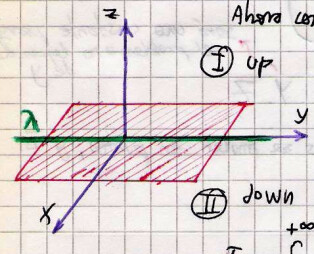
\includegraphics[width=0.4\textwidth]{images/fig_ft1_problema2_sep_C.jpg}

Se propone una fórmula 
\[
	\phi = X Y Z,
\]
donde $X$ es una $\euler^{ikx}$, $Y$ es una constante y para $Z$
se toma $ \sinh( k |z - a/2| ) $ porque un solo cero es necesario.
Entonces tenemos prescripciones para cada zona que son 
\[
	\phi_I = \int_{-\infty}^{\infty} \: 
	\sinh( k|z-a/2| ) \: A_k^I \: \euler^{ikx} \: dk
\]
\[
	\phi_{II} = \int_{-\infty}^{\infty} \: 
	\sinh( k|z-a/2| ) \: A_k^{II} \: \euler^{ikx} \: dk
\]

Entonces, de la evaluación de los contornos 
\[
	\phi_I(z=0) = \phi_{II}(z=0)
\]
surgen
\[
	A_k^{I} = A_k^{II} \equiv A_k
\]
y asimismo
\[
	- 2 \int A_k \euler^{ikx} k \cosh( ka/2 ) \: dk 
	- 2 \int A_k \euler^{ikx} k \cosh( ka/2 ) \: dk = 4 \pi \lambda \delta(x)
\]
lo cual nos lleva a
\[
	- 2 \int A_k \euler^{ikx} k \cosh( ka/2 ) \: dk
	= 4 \pi \lambda \delta(x),
\]
y multiplico por $\int \euler{-ik'x} dx$
\notamargen{
Usaremos la expresión de la delta en Fourier:
\[
	2 \pi \delta(k-k') = \int \: \euler^{ i (k - k') x} \: dx
\]}
lo cual lleva a 
\[
	A_k = \frac{-\lambda}{k'\cosh(ka/2)},
\]
y volviendo todo a $k$ sin primar
\[
	\phi = -\lambda \int dk \: \euler^{ikx} \:
	\frac{\sinh( k|z-a/2|)}{k'\cosh(ka/2)}
\]

Para este caso obtenemos para el potencial una integral, contrariamente
a lo que teníamos para el otro caso donde aparecía una serie.

Queremos ver la relación entre ambas,
\[
	\sinh( k |z-a/2 |) = \sum_{n} A_n \cos(k_n z)
\]
Sacamos de una tabla la forma del $A$, que es
\[
	A_n = - \frac{4k}{a} \frac{\cosh( ka/2 )}{ ( k^2 + k_n^2 ) }
\]
y obtenemos, a menos de una constante,
\[
	\int \frac{ \euler^{ i k x } }{ ( k^2 + k_n^2 ) } \: dx
\]
Por residuos se tiene 
\[
	\int \frac{ \euler^{ i k x } }{ ( k - i k_n )( k + i k_n ) } \: \mathrm{Res}(f, \text{den.})
\]

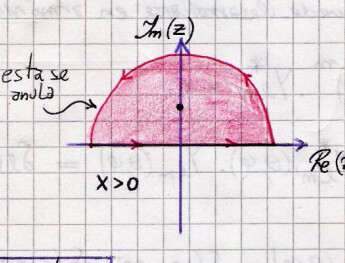
\includegraphics[width=0.4\textwidth]{images/fig_ft1_problema2_sep_D.jpg}

Usamos residuos para evaluar la integral. Vemos que da
\[
	\frac{2 \pi i \euler^{-k_n} }{ 2 i k_n }
\]

En el caso de $x>0$ se tendrá
\[
	\phi = 4 \lambda \sum_n \frac{\cos(k_nz)}{2n +1} \euler^{- k_n x}
\]

Para calcular las cargas inducidas, véase figurin bajo estas líneas, será

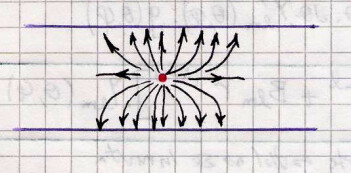
\includegraphics[width=0.4\textwidth]{images/fig_ft1_problema2_sep_E.jpg}

\[
	\left. \dpar{\phi^{II}}{z} \right|_{z=-a/2} = 4 \pi \sigma_{\text{ind}}
\]
donde
\[
	\sigma = \frac{ \lambda \euler^{ \pi |x|} }{a( 1 + \euler^{-})} 
\]
y entonces
\[
	\int \sigma dx = \frac{Q^{\text{ind}}}{L} = - \frac{\lambda}{2}
\]

\end{ejemplo}



Lo que sucede en las direcciones x, y son condiciones periódicas de potencial que requieren
dos ceros.
% Se da que $A_{m,n}$ es una constante general y hay condiciones periódicas en $x,y$
% \[
% 	A\euler^{\pm i\alpha x} = A_\alpha \cos(\alpha x) + B_\alpha \sin(\alpha x)
% \]
% corresponde a condiciones de potencial periódicas, cuando necesito dos ceros por ejemplo (ver ilustración
% lateral --que falta--)
% \[
% 	A\euler^{\pm \gamma z} = A_\gamma \cosh(\gamma z) + B_\gamma \sinh(\gamma z)
% \]
% corresponde a atravesar densidades de carga.

\section{Separación en coordenadas esféricas}

Para coordenadas esféricas es
\[
	\frac{1}{r} \frac{\partial}{\partial r}\left( r^2 \dpar{\phi}{r} \right) + 
	\frac{1}{r^2 \sin(\theta)}\frac{\partial}{\partial\theta}\left(\sin(\theta)\dpar{\phi}{\theta}\right)+
	\frac{1}{r^2 \sin(\theta)} \dpar[2]{\phi}{\varphi} = 0
\]
proponiéndose la separación
\[
	\phi(r,\theta,\varphi) = R(r) \: \Theta(\theta) \: Q(\varphi)
\]
resulta en 
\[
	\frac{\sin^2\theta}{R} \dtot{}{r}\left( r^2 \dtot{R}{r} \right) + 
	\frac{\sin\theta}{\Theta} \dtot{}{\theta}\left( \sin(\theta)\dtot{\Theta}{\theta}\right) =
	- \frac{1}{Q} \dtot[2]{Q}{\vp} 
\]
\notamargen{Las coordenadas convenientes dependerán de los contornos.
Recordemos que siempre la cosa es resolver la ecuación más sus BC.}
Procediendo como en el caso anterior, se tiene primeramente
\[
	\frac{1}{Q} \dtot[2]{Q}{\vp} = - \alpha^2,
\]
un oscilador armónico en $\vp$ de manera que 
\[
	Q = \euler^{\pm i\alpha \varphi},
\]
donde en principio $\alpha \in \mathbb{R}$ pero podemos ir más lejos y como 
\[
	\cos \alpha\vp = \cos (\alpha\vp \pm 2\pi)
\]
se sigue que $\alpha \in \mathbb{Z}$ y podemos llamarlo $m^2 \equiv \alpha^2 \in \mathbb{Z}$.
Estamos suponiendo que tenemos un recinto de integración que abarca todo el rango de $\vp$
de $0$ a $2\pi$. Debe tenerse presente que esta solución no sirve si la distribución no
abarca todo el intervalo angular mencionado.

Luego,
\[
	- \frac{1}{\Theta \sin\theta } \dtot{}{\theta}\left( \sin(\theta)\dtot{\Theta}{\theta}\right) +
	\frac{m^2}{\sin^2\theta} = \beta^2,
\]
que merced al cambio de variables $x = \cos\theta$, que implica $d/d\theta = - \sin\theta d/dx$ lleva
la ecuación anterior a la forma
\[
	\dtot{}{x}\left[ (1-x^2)\dtot{\Theta}{x} \right] + \left[ \beta^2 - \frac{m^2}{1-x^2} \right] \Theta = 0,
\]
la cual es claramente un problema de Sturm-Liouville. Con respecto a $r$ se tiene
\[
	\frac{1}{R} \dtot{}{r}\left( r^2 \dtot{R}{r} \right) = \beta^2
\]
donde un nuevo cambio de variables $R(r) = U(r)/r$ conduce a
\[
	\dtot[2]{U}{r} - \frac{\beta^2 U }{r^2}= 0
\]

Si el problema tiene simetría azimutal ($m=0$) se tendrá\footnote{Si $m=0$ significa sencilamente
que no depende del ángulo $\vp$, o sea que hay simetría de revolución.}:
\be
	\dtot{}{x}\left[ (1-x^2)\dtot{P}{x} \right] + \beta^2 P = 0,
	\label{sep_spherical_P}
\ee
la cual tiene un punto singular en $x^2=1$ que corresponde al coseno en $0$ o en $\pi$ (el eje polar).
Este problema se evita con 
\be
	\beta^2 = \ell ( \ell + 1 ), \qquad \ell \in \mathbb{N}
	\label{cond_pol_lag}
\ee
porque la serie sólo se mueve entre $z \in (-1,1)$ y entonces con la condición \eqref{cond_pol_lag} las funciones
aque salen de la ecuación \eqref{sep_spherical_P} no presentan singularidades.
La serie que da $P$ se corta. Son los polinomios de Legendre. Tenemos una nueva restricción entonces que es el
eje polar $-1<z<1$. Se reescribe la \eqref{sep_spherical_P} como
\[
	\dtot{}{x}\left[ (1-x^2)\dtot{P}{x} \right] +  \ell ( \ell + 1 ) P = 0.
\]

Las funciones $P$ son los polinomios de Legendre $P_\ell$ que forman un conjunto completo y son ortogonales
entre sí. Se pueden construir con la fórmula de Rodrigues
\[
	P_\ell (x) = \frac{1}{2^\ell \ell!} \frac{d^\ell}{d x^\ell} [x^2 - 1]^\ell, 
\]
donde se cumple $P_\ell(x=1) = 1$ y además las condiciones de ortogonalidad son
\[
	\int_{-1}^{+1} P_{\ell'}(x) P_\ell (x) \: dx= \frac{2}{2\ell + 1} \: \delta_{\ell\ell'}
\]
Se ve [¿?]
\[
	(\ell+1) P_{\ell+1} - (2\ell+1) x P_{\ell} + \ell P_{\ell-1} = 0
\]
\[
	\dtot{P_{\ell+1}}{x} - x \dtot{P_{\ell}}{x} - (\ell+1) P_{\ell} = 0
\]
\[
	(x^2-1) \dtot{P_{\ell}}{x} - \ell x P_{\ell} + \ell P_{\ell-1} = 0
\]
y
\[
	\dtot[2]{U}{r} - \frac{\ell(\ell+1)}{r^2} U = 0
\]
de manera que su solución será del tipo
\[
	U(r) = A r^{\ell+1} + B R^{-\ell}.
\]

siendo
\[
	Y(\theta,\varphi) = \Theta(\theta) Q(\varphi)
\]
un armónico esférico.


si usamos $0\leq \varphi \leq 2\pi$ de modo que $\alpha\in\mathbb{Z}$ y entonces $\alpha=m$, con simetría
azimutal es $m=0$ (rotación en $\varphi$), 
\[
	Q = G\varphi + H \qquad\qquad  G,H \quad ctes.
\]
Para las otras funciones será
\[
	R(r) = A_\ell r^\ell + B_\ell R^{-\ell-1}
\]
\[
	\Theta(\theta) = C_\ell P_\ell^m (\cos(\theta)) + D_\ell Q_\ell^m (\cos(\theta))
\]
siendo $P_\ell^m$ polinomio de Legendre, que verifica la fórmula de Rodrigues
\[
	P_\ell (x) = \frac{1}{2^\ell \ell!} \frac{d^\ell}{d x^\ell} [x^2 - 1]^\ell
\]
con $P_\ell(\cos(\theta))$ polinomio de Legendre de primera especie, y $Q_\ell(\cos(\theta))$ de segunda
especie.
Los $\{ P_\ell\}$ son un conjunto completo y ortogonal en $-1 \leq x \leq 1$ o bien en $0\leq \theta\leq \pi$.

Los $\{ Q_\ell^m(\cos(\theta))\}$ tienen problemas en $\theta=0,\theta=\pi$ (eje $z$) de manera que si está el
eje $z$ no podemos usar $Q_\ell^m$; en estos problemas sólo podemos usar $P_\ell^m(\cos(\theta))$.
Luego, la solución total será
\[
	\phi(r,\theta,\phi) = [ \: R(r) \: ] [ \: \Theta(\theta) \: ] [ \: Q(\vp) \: ],
\]
o bien
\[
	\phi(r,\theta,\phi) = \sum_{\ell=0}^{\infty}\sum_{m=-\infty}^{\infty} \left[ A_\ell r^\ell + 
	B_\ell r^{-\ell-1} \right] \left[ C_\ell P_\ell^m + D_\ell Q_\ell^m \right] \left[ E_m \cos(m\phi) + 
	F_m \sin(m\phi) \right]
\]
y en el caso particular $m=0$
\[
	\phi(r,\theta,\phi) = \sum_{\ell=0}^{\infty}\sum_{m=-\infty}^{\infty} \left[ A_\ell r^\ell + 
	B_\ell r^{-\ell-1} \right] \left[ C_\ell P_\ell^m + D_\ell Q_\ell^m \right] \left[ G_0 \phi + 
	H_0 \right]	
\]
Las constantes $A_\ell, B_\ell, C_\ell, D_\ell, E_m, F_m$ se ajustan con el $\phi (r\to\infty)$, 
$\phi (r\to 0)$, $\phi (z = 1)$ y $\phi (z = -1)$.

Lo que permite esquivar el problema del punto singular en $x \equiv \cos(\theta)=1$ es
\[
	\beta^2 = \ell(\ell + 1) \qquad - \ell < m < \ell \qquad \alpha^2 = m^2
\]

Recordemos las sumas de series
\[
	\frac{1}{1-z} = \sum_{\ell=0}^{\infty} z^\ell \qquad \frac{1}{1+z} = \sum_{\ell=0}^{\infty} (-1)^\ell 
	z^\ell	\qquad |z|<1,
\]
el polinomio asociado de Legendre
\[
	P_\ell^m (x) =) \frac{(-1)^m}{2^\ell \ell!} [1-x^2]^{m/2} \frac{d^{\ell + m}}{dx^{\ell + m}} 
			[x^2 -1]^\ell
\]
que cumple
\[
	P_\ell (1) = 1 \qquad  \qquad P_\ell (-1) = (-1)^\ell \qquad  \forall \ell
\]
con 
\[
	\int_{-1}^1 [P_\ell (x)]^2 \: dx = \frac{2}{ 2\ell + 1 }
\]
siendo la ortogonalidad
\[
	\int_0^\pi P_{\ell'}^m (\cos(\theta)) P_\ell^m (\cos(\theta)) \sin(\theta) \: d\theta = 
	\delta_{\ell\ell'}
\]
\[
	\int_{-1}^{+1} P_{\ell'}^m (x) P_\ell^m (x) \: dx= \frac{2}{2\ell + 1}
	\frac{(\ell + m)!}{(\ell - m)!} \: \delta_{\ell\ell'}
\]

En esféricas las constantes de separación están asociadas
\[
	R(r) \; \mathrm{con} \; \ell \qquad \Theta(\theta) \; \mathrm{con} \; \ell,m \qquad
	Q(\phi) \; \mathrm{con} \; m
\]


\begin{ejemplo}{\bf Problema de separación esférica}

Ya este problema, ver figura, tiene simetría de revolución. Entonces será $m = 0$ 

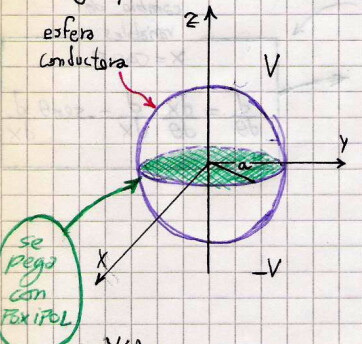
\includegraphics[width=0.4\textwidth]{images/fig_ft1_ejemplo_sep_sphe_A.jpg}

\be
	\vp(r,\theta) = \sum_{\ell=0}^\infty \: \left[ 
	A_\ell r^\ell + B_\ell r^{-(\ell+1)}
	\right] P_\ell \cos\theta
	\label{potencial_azimutal}
\ee
En dos secciones diferentes se tendrá
\[
	r> a \qquad \quad 
		\vp_I(r,\theta) = \sum_{\ell=0}^\infty \: 
	B_\ell r^{-(\ell+1)} P_\ell \cos\theta
\]
\[
	r< a \qquad \quad 
	\vp(r,\theta) = \sum_{\ell=0}^\infty \:
	A_\ell r^\ell P_\ell \cos\theta
\]

Entonces, cada potencial tiende al valor $V(x)$
\[
	\vp_I(r,\theta)_{r=a} \to V(x) \qquad 
	\vp_{II}(r,\theta)_{r=a} \to V(x)
\]

El escalón refleja la imparidad, de manera que sólo aparecerán
términos impares. Ahora queremos desarrollar el escalón en
polinomios de Legendre

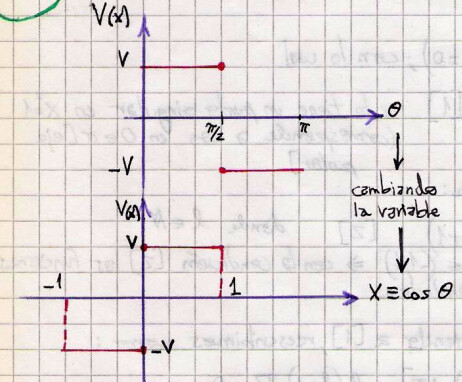
\includegraphics[width=0.4\textwidth]{images/fig_ft1_ejemplo_sep_sphe_B.jpg}

El gráfico de arriba tiene también el cambio de variables $x\equiv \cos\theta$,
\[
	\frac{V(x)}{V} = \sum_{\ell=0}^\infty \: c_\ell P_\ell 
\]
con $\ell$ impar. El coeficiente 
\[
	c_\ell = \frac{2\ell + 1}{2} \: \int_{-1}^{1} P_\ell (x) \: dx
	= ( 2 \ell + 1 ) \int_{0}^{1} P_\ell (x) \: dx,
\]
y usando la fórmula de Rodrigues
\[
	c_\ell = \frac{2\ell + 1}{2^\ell \ell! } \: 
	\int_{0}^{1} \: \dtot[\ell]{ ( x^2 - 1 )^\ell }{x} \: dx
\]
se viene 
\[
	c_\ell = \Frac{-1}{2}^{(\ell -1)/ 2}
	\frac{(2\ell +1)(\ell -2)!!}{2((\ell+1)/2)!}
\]
donde el doble factorial es sobre los impares. Hemos hallado los coeficientes.
Reemplazando para los primeros
\[
	c_1 = 3/2 \qquad c_3 = -7/8 \qquad c_5 = 11/16,
\]
Entonces 
\[
	A_\ell = V a^{-\ell} c_\ell \qquad \qquad 
	B_\ell = V a^{\ell+1} c_\ell
\]

\end{ejemplo}




% =================================================================================================
\section{Detalles sobre solución de problemas de potencial}
% =================================================================================================

Si el potencial es par en una coordenada, entonces uso funciones pares (cosenos). 
La continuidad del potencial
\[
	\phi_I(x=0) = \phi_{II}(x=0) = 
\]
y salto en el campo
\[
	\left.\dpar{\phi_I}{x} - \dpar{\phi_{II}}{x}\right|_{x=0} = -4\pi\sigma|_{x=0}
\]

\begin{figure}[htb]
	\begin{center}
	\includegraphics[width=0.4\textwidth]{images/fig_ft1_potencial.pdf}	 
	\end{center}
	\caption{}
\end{figure} 
Si tengo condiciones periódicas en la coordenada irán senos y cosenos trigonométricos, entonces se
discretizan $m,n$ y tengo $\sum_n \sum_m$ una serie de Fourier.

Si tengo condiciones no periódicas en la coordenada irán seno, coseno hiperbólicos entonces tengo
$\int dk$ integral de Fourier.

En general tomo
\[
	\alpha^2 + \beta^2 = \gamma^2
\]
pudiéndose discretizar los $k's$ luego. Se considera $\alpha^2 \equiv k_{\hat{e}_1}^2$ y así siguiendo
con las otras dos.

Sobre la ecuación de salto en el campo aplicamos ortogonalidad y despejamos coeficientes en función
de $\sigma$.

Detalle: el salto en el campo se hace siguiendo la normal, como se ilustra abajo
\begin{figure}[htb]
	\begin{center}
	\includegraphics[width=0.3\textwidth]{images/fig_ft1_potencialsketch.pdf}
	\end{center}
	\caption{}
\end{figure} 
\[
	E_I^{\hat{n}} - E_{II}^{\hat{n}} = 4 \pi \sigma \qquad\qquad 
	- \dpar{\phi_I}{x} + \dpar{\phi_{II}}{x} = 4 \pi \sigma
\]

Para $k_{\hat{e}_1}^2$ en el caso discreto
\[
	\sum_{m=0}^\infty \cos(k_m e_1) + \sin(k_m e_1)
\]
pero en el continuo 
\[
	\int_{\infty}^{\infty} \euler^{ike_1} dk
\]
usamos $exp(ike_1)$ para que la integral converja en lugar de $(\cos(ke_1) + \sin(ke_1))$.

\subsection{Desarrollo distancia entre puntos}

\begin{figure}[thb]
	\begin{center}
	\includegraphics[width=0.4\textwidth]{images/fig_ft1_expansiones1.pdf}	 
	\end{center}
	\caption{}
\end{figure} 

Es útil el desarrollo
\[
	\frac{1}{|\vb{r} - \vb{r}'|} = \frac{1}{\sqrt{r^2 + r'^2 -2rr'\cos(\gamma)}}
	= \sum_{\ell=0}^\infty \frac{r^\ell_{<}}{r^\ell_{>}} P_\ell (\cos(\gamma))
\]
en polinomios de Legendre para el ángulo entre vectores en coordenadas esféricas.
En coordenadas esféricas, donde $\gamma=\gamma(\theta,\phi)$ es el ángulo entre vectores,
que surge del teorema del coseno.

\subsection{Prolongación analítica}

Consiste en {\it prolongar} una solución restringida por ejemplo en el eje polar a todo el
resto del espacio pegándole los polinomios de Legendre.

Como ejemplo vemos un anillo con carga $Q$ distribuida uniformemente. Hay un plano
de simetría perpendicular al eje de simetría.

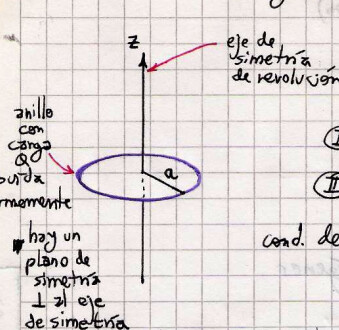
\includegraphics[width=0.3\textwidth]{images/fig_ft1_prolongacion_A.jpg}

A partir de la prescripción \eqref{potencial_azimutal}
\[
	r > a \quad \vp_1(\vbx) = \sum_{n=0}^{\infty} B_{2n} r^{-(2n+1)} P_{2n}( \cos\theta )
\]
\[
	r < a \quad \vp_2(\vbx) = \sum_{n=0}^{\infty} A_{2n} r^{2n} P_{2n}( \cos\theta )
\]
y hay que ver las condiciones de contorno. Me quedaré con los coeficientes
pares porque es simétrico el potencial por la simetría en $\theta$,

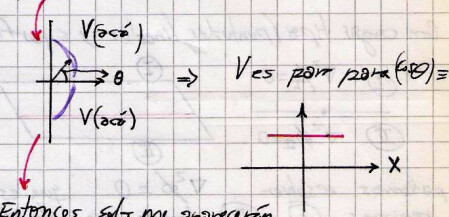
\includegraphics[width=0.3\textwidth]{images/fig_ft1_prolongacion_B.jpg}

y por ello sólo me aparecerán coeficientes pares.
Los potenciales están evaluados en el eje polar que son dos ángulos theta,
\[
	\vp_1(\theta=0^\circ,180^\circ) = 
	\sum_{n=0}^{\infty} \: B_{2n} r^{-(2n + 1)} \qquad
	\vp_2(\theta=0^\circ,180^\circ) = 
	\sum_{n=0}^{\infty} \: A_{2n} r^{2n}
\]
una serie de potencias para el potencial $V(\vbx = \zver)$ de un anillo (que
es un caso ya resuelto en F3).

Luego, multiplicando esta serie de potencias por los polinomios de Legendre
tendremos el $V$ para todo el espacio.
El cálculo elemental da
\[
	\vp(\vbx)(\theta=0^\circ,180^\circ) = \frac{Q}{\sqrt{r^2 + a^2}} =
	\frac{Q}{r \sqrt{1 + a^2 / r^2 }}
\]
Entonces
\[
	\vp_1(\theta=0^\circ,180^\circ) =
	\frac{Q}{r} \sum_{n=0}^{\infty} \: (-1)^n \Frac{a}{r}^{2n}
	\frac{(2n-1)!!}{2^n n!}
\]
\[
	\vp_2 =
	\frac{Q}{a} \sum_{n=0}^{\infty} \: (-1)^n \Frac{r}{a}^{2n}
	\frac{(2n-1)!!}{2^n n!}
\]

Ahora para todo el espacio es
\[
	\vp_1(r>a) =
	\frac{Q}{r} \sum_{n=0}^{\infty} \: (-1)^n \Frac{a}{1}^{2n}
	\frac{(2n-1)!!}{2^n n!} \: r^{-2n} \: P_{2n}( \cos\theta )
\]
\[
	\vp_2(r<a) =
	\frac{Q}{a} \sum_{n=0}^{\infty} \: (-1)^n \Frac{r}{a}^{2n}
	\frac{(2n-1)!!}{2^n n!} \: \: P_{2n}( \cos\theta )
\]

En notación compacta
\[
	\vp(\vbx) = Q \sum_{n=0}^{\infty} \: (-1)^n \frac{(2n-1)!!}{2^n n!}
	\Frac{r_<}{r_>}^{2n+1} \: P_{2n}(\cos\theta) .
\]

\notamargen{A partir de aquí están los barruntos de las notas de final. Habría
que consolidar con lo transcripto desde la carpeta.}
Lo ponemos en serie (pasamos un cálculo de F3 a una serie)
\[
	\phi(r,\phi/2) = \frac{Q}{\sqrt{r^2 + a^2}} = \sum_{\ell=0}^\infty Q \frac{a^\ell}{r^{\ell + 1}} 
	P_\ell (0) \qquad r > a
\]
\[
	\phi(r,\phi/2) = \frac{Q}{\sqrt{r^2 + a^2}} = \sum_{\ell=0}^\infty Q \frac{r^\ell}{a^{\ell + 1}} 
	P_\ell (0) \qquad r < a
\]
y $P_\ell(0)$ tiene términos pares solamente (los impares son nulos).

\begin{figure}[htb]
	\begin{center}
	\includegraphics[width=0.3\textwidth]{images/fig_ft1_expansiones2.pdf}	 
	\end{center}
	\caption{}
\end{figure} 

Entonces
\[
	\phi(r,\phi/2) = \frac{Q}{a} \sum_{n=0}^\infty \frac{r^{2n}}{a^{2n}} P_{2n} (0) 
\]
con 
\[
	P_{2n} (0) = (-1)^n \frac{(2n-1)!}{2^n n!}
\]
por lo tanto para todo el espacio será

\begin{figure}[htb]
	\begin{center}
	\includegraphics[width=0.4\textwidth]{images/fig_ft1_expansiones3.pdf}	 
	\end{center}
	\caption{}
\end{figure} 

\[
	\phi(r,\phi/2) = \frac{Q}{a} \sum_{n=0}^\infty \left( \frac{r}{a}\right)^{2n} P_{2n} (0) P_{2n} 
	(\sin(\theta)) \qquad r < a
\]
El hecho de que sólo vivan $\ell$ pares viene porque $\phi$ es par pues hay simetría de reflexión en el
plano $xy$, lo que sucede de $(0,\pi/2)$ es igual a lo que sucede de $(\pi/2, \pi)$.

Los problemas con simetría de revolución en torno a $\hat{z}$ pueden ser resueltos con el método de
prolongación analítica. La idea central es que si dos soluciones del potencial coinciden en un conjunto
de puntos (como ser el eje azimutal) entonces deben ser la misma solución.

\subsection{Comentario multipolos}

Estos dos problemas son equivalentes, pero multipolarmente tienen desarrollos diferentes.
El problema es que el metal a tierra tendrá carga hasta el infinito y entonces no podemos tener un
radio de convergencia.

\begin{ejemplo}{\bf Problema esfera y aro}

La situación del problema puede verse en la ilustración dada por el figurín siguiente

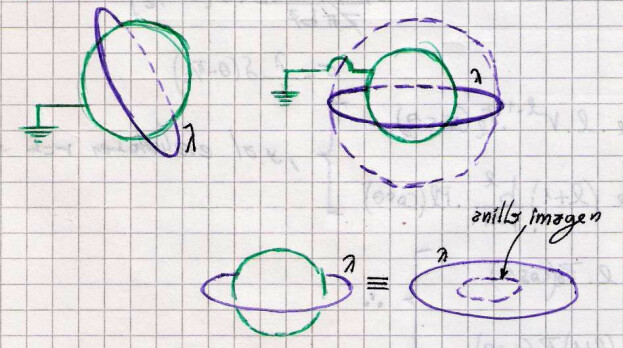
\includegraphics[width=0.5\textwidth]{images/fig_ft1_problema_esfera_anillada_A.jpg}

La situación física que se observa qes que habrá simetría azimutual, dado que la distribución
es la misma para todo ángulo $\vp$. Entonces será $m=0$.
Además, como el eje polar forma parte de la solución también se descartará $Q^m_\ell$
dado que se necesita regularidad en $-1,1$.

Entonces, el candidato es
\[
	\phi^{I,II} = \sum_\ell \: ( A_\ell^{I,II} r^\ell + B_\ell^{I,II} r^{-\ell-1}) P_\ell(\cos\theta)
\]
donde hemos establecido las dos regiones ilustradas aquí abajo

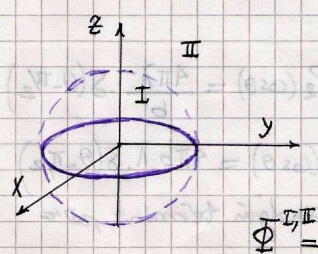
\includegraphics[width=0.4\textwidth]{images/fig_ft1_problema_esfera_anillada_B.jpg}

Luego, requeriremos regularidad en $r \to \infty$ para $\phi^{II}$ y en $r=0$ para $\phi^{I}$
lo cual conduce a
\[
	A_\ell^{II} = 0 \qquad B_\ell^{I} = 0
\]

Entonces
\[
	\phi^{I} = \sum_\ell \: A^I_\ell \: r^\ell \: P_\ell(\cos\theta) \qquad \qquad 
	\phi^{II} = \sum_\ell \: B^{II}_\ell \: r^{-\ell-1} \: P_\ell(\cos\theta)
\]
y del contorno en $b$ se tiene
\[
	\phi^{I}(r=b) = \phi^{II}(r=b) = \qquad 
	A^{I}_\ell \: b^{-\ell-1} = B^{II}_\ell \: b^{-\ell-1} \equiv \frac{C_\ell}{b}
\]
\[
	\phi^{I} = \frac{1}{b} \: \sum_\ell \: C_\ell \: \Frac{r}{b}^{\ell} \: P_\ell(\cos\theta) \qquad\qquad 
	\phi^{II} = \frac{1}{r} \: \sum_\ell \: C_\ell \: \Frac{b}{r}^{\ell} \: P_\ell(\cos\theta)
\]

El análisis de $\rho(r,\theta,\vp)$ tal que $\int \rho dV = q$ en principio nos dice que no 
dependerá de $\vp$ y tendremos una forma
\[
	\rho = f(\theta) \delta(r-b) \qquad \rho = \alpha(r,\theta) \delta(\theta-\pi/2) \delta(r-b)
\]
la cual por integración
\[
	\rho = \frac{q}{2 \pi r^2 \sin \theta } \: \delta(\theta-\pi/2) \delta(r-b)
\]
\notamargen{En este caso el $\sin\theta$ podría no estar [¿?].}
lo cual conduce a una 
\[
	\sigma = \frac{\lambda}{b} \: \delta(\theta-\pi/2)
\]

Las derivadas del potencial serán
\[
	\dpar{\phi^{I}}{n} = \dpar{\phi^{I}}{r} = 
	\frac{1}{b} \: \sum_\ell \: C_\ell \: \ell \: \Frac{r}{b}^{\ell-1} b \: P_\ell(\cos\theta) 
\]
\[
	\dpar{\phi^{II}}{n} = \dpar{\phi^{II}}{r} =
	- \frac{1}{r} \: \sum_\ell \: C_\ell \: {\ell+1} \: \Frac{b}{r}^{\ell+1} \: b^{-1} \: P_\ell(\cos\theta)
\]
y al evaluarlas en $r=b$
\[
	\left.\dpar{\phi^{I}}{r} \right|_b = 
	\frac{1}{b^2} \: \sum_\ell \: C_\ell \: \ell \: P_\ell(\cos\theta) 
	\qquad 
	\left.\dpar{\phi^{II}}{r} \right|_b =
	- \frac{1}{b^2} \: \sum_\ell \: C_\ell \: (\ell+1) \: P_\ell(\cos\theta)
\]
por lo tanto
\[
	 \left. -\left( \dpar{\phi^{II}}{n} - \dpar{\phi^{I}}{n} \right) \right|_b =
	 \frac{1}{b^2} \: \sum_\ell \: C_\ell \: (2\ell+1) \: P_\ell(\cos\theta) = 
	 \frac{4\pi \lambda}{b} \delta(\theta-\pi/2)
\]
\[
	\sum_\ell \: C_\ell \: (2\ell+1) \: P_\ell(\cos\theta) = 
	4\pi \lambda b \delta(\theta-\pi/2)
\]
y ahora necesitaríamos encontrar $C_\ell$ para lo cual multiplicaremos ambos miembros
y haremos uso de las condiciones de ortogonalidad de los polinomios [ver equaciones
tal y tal]
\[
	\sum_\ell \: C_\ell \: (2\ell+1) \: \int_0^\pi \sin\theta P_{\ell'}(\cos\theta) P_\ell(\cos\theta) d\theta = 
	4\pi \lambda b \int_0^\pi \sin\theta P_{\ell'}(\cos\theta) \delta(\theta-\pi/2) d\theta
\]
que resulta en
\[
	C_{\ell'} \: (2\ell'+1) \frac{2}{2\ell'+1} = 
	4\pi \lambda b \: P_{\ell'}(0)
\]
y de lo cual se desprende que ahora podemos escribir
\[
	\phi^{I} = 2\pi\lambda \: \sum_\ell \: \Frac{r}{b}^{\ell} \: P_{\ell}(0) \: P_\ell(\cos\theta) 
	\qquad \qquad 
	\phi^{II} = 2\pi\lambda \: \sum_\ell \: \Frac{b}{r}^{\ell+1} \: P_{\ell}(0) \: P_\ell(\cos\theta)
\]

Luego,
\[
	P_{\ell+1}(x) (\ell+1) - (2\ell+a) x P_{\ell}(x) + \ell P_{\ell-1}(x) = 0
\]
y para sucesivos
\[
	P_{\ell+1}(0) (\ell+1) + \ell P_{\ell-1}(0) = 0 \qquad 
	P_{\ell+2}(0) (\ell+2) + (\ell+1) P_{\ell}(0) = 0
\]
\[
	P_{\ell+2}(0) = -\frac{(\ell+1)}{(\ell+2)} P_{\ell}(0)
\]
\[
	P_0(x) = 1 \qquad P_1(x) = x \qquad \qquad 
	P_0(0) = 1 \qquad P_1(0) = 0
\]
y se ve que los $P_\ell$ que aportarán serán los pares, de manera que
\[
	P_{2}(0) = -\frac{1}{2} \qquad 
	P_{4}(0) = \left( -\frac{3}{4}  \right) \left( -\frac{1}{2}  \right)\qquad 
	P_{6}(0) = \left( -\frac{5}{6}  \right)\left( -\frac{3}{4}  \right) \left( -\frac{1}{2}  \right)
\]
\[
	P_{2n}(0) = (-1)^n \frac{(2n-1)!!}{(2n)!!}
\]
tras lo cual
\[
	\phi^{I} = 2\pi\lambda \: \sum_n \: (-1)^n \frac{(2n-1)!!}{(2n)!!} 
	\: \Frac{r}{b}^{2n} \: P_{2n}(\cos\theta) 
\]
\[
	\phi^{II} = 2\pi\lambda \: \sum_n \: (-1)^n \frac{(2n-1)!!}{(2n)!!} 
	\: \Frac{b}{r}^{2n+1} \: P_{2n}(\cos\theta)
\]

Ahora se {\it mete} a tierra la esfera por imágenes, ver ilustración siguiente

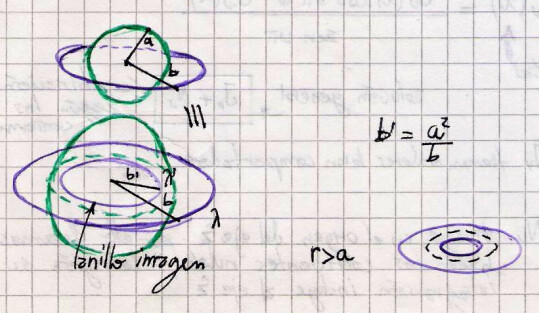
\includegraphics[width=0.45\textwidth]{images/fig_ft1_problema_esfera_anillada_C.jpg}

Con ello
\[
	\lambda = \frac{dq}{b \: d\theta} \qquad \lambda' = \frac{dq'}{b' \: d\theta}
\]
y
\[
	\lambda'= -\frac{b}{a}\lambda.
\]

Deberíamos obtener, si hacemos la superposición,
\[
	\phi^{I} = 2\pi\lambda \: \sum_n \: (-1)^n \frac{(2n-1)!!}{(2n)!!} 
	\: \Frac{ r^{4n+1} - a^{4n+1} }{ r^{2n+1} b^{2n} } \: P_{2n}(\cos\theta) 
\]
\[
	\phi^{II} = 2\pi\lambda \: \sum_n \: (-1)^n \frac{(2n-1)!!}{(2n)!!} 
	\: \Frac{ b^{4n+1} - a^{4n+1} }{r^{2n+1} b^{2n} } \: P_{2n}(\cos\theta)
\]

También se puede llegar directamente a la resolución por seperación de variables en
la configuración

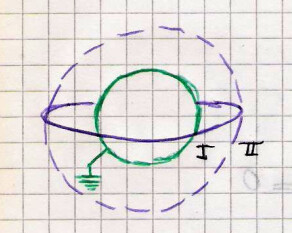
\includegraphics[width=0.3\textwidth]{images/fig_ft1_problema_esfera_anillada_D.jpg}

Es similar de entrada
\[
	\phi^{I,II} = \sum_\ell \: ( A_\ell^{I,II} r^\ell + B_\ell^{I,II} r^{-\ell-1}) P_\ell(\cos\theta).
\]


\end{ejemplo}



% =================================================================================================
\section{Armónicos esféricos}
% =================================================================================================

Considérese el problema de Sturm-Liouville siguiente
\[
	\dtot{}{x} \left[ (1-x^2) \dtot{P}{x} \right] + \left[ e(e+1) - \frac{m^2}{1-x^2} \right] P = 0
\]
para $ 0 \leq \vp \leq 2\pi$ y $-1 \leq x \leq 1$. Como $ \ell \geq 0$ y $ -\ell \leq m \leq \ell$
se tendrán 
\[
	P_{\ell m} = (-1)^m (1-x)^{m/2} \dtot[m]{}{x} P_\ell(x) =
	\frac{(-1)^m}{2^\ell \ell!} (1-x)^{m/2} \dtot[{\ell+m}]{}{x} (x^2-1)^\ell
\]
y entonces
\[
	P_{\ell, -m} = (-1)^m \frac{(\ell -m)!}{(\ell + m)!} P_{\ell m}(x)
\]
con $\phi_m = \euler^{im\vp}$.
La condición de ortogonalidad nos dice que
\[
	\int_{-1}^1  P_{\ell' m}(x) \: P_{\ell m}(x) \: dx = 
	\frac{2}{2\ell +1} \frac{(\ell + m)!}{(\ell - m)!} \delta_{\ell\ell'}
\]
y de lo cual deducimos que 
\[
	 P_{\ell m}(x)\phi_m(x).
\]
Estas expresiones se presentan en forma conjunta y normalizada. Son los armónicos
esféricos.
\[
	Y_{\ell,m}(\theta,\varphi) = \sqrt{ \frac{ 2\ell + 1}{4\pi} \frac{(\ell-m)! }{(\ell+ m)! } }
	P_\ell^m(\cos(\theta)) \euler^{i m \varphi}
\]
Los armónicos esféricos son un conjunto ortonormalizado en 
\notamargen{En la carpeta tenía $x$ en lugar de $\cos(\theta)$.}
\[
	- 1 \leq \cos(\theta) \leq 1 , \qquad 0 \leq \varphi \leq 2\pi
\]

Se verifica también
\[
	Y_{\ell,-m}(\theta,\varphi) = (-1) Y_{\ell,m}^*(\theta,\varphi).
\]

La ortonormalidad es
\[
	\int_0^{2\pi} d\varphi \int_0^\pi \sin(\theta) 
	Y_{\ell,m}(\theta,\varphi) Y_{\ell,m}^*(\theta,\varphi) d\theta 
	= \delta_{\ell'\ell}\delta_{m'm}
\]
mientras que la completitud
\[
	\sum_{\ell=0}^\infty \sum_{m=-\ell}^\ell Y_{\ell,m}(\theta,\varphi) Y_{\ell,m}^*(\theta,\varphi) = 
	\delta(\varphi 	-\varphi') \delta(\cos(\theta)-\cos(\theta'))
\]
nos dice que solo es diferente de cero esta suma cuando los ángulos primados y 
sin primar son iguales.
Entonces una función $f$ cualquiera $\in L^2$ se puede expresar en armónicos esféricos,
\[
	f(\theta,\varphi) = \sum_{\ell=0}^\infty \sum_{m=-\ell}^\ell A_{\ell,m} Y_{\ell,m}(\theta,\varphi)
\]
donde 
\[
	A_{\ell,m} = 	\int_0^{2\pi} d\varphi \int_0^\pi \sin(\theta) f(\theta,\vp)
	Y_{\ell,m}(\theta,\varphi) Y_{\ell,m}^*(\theta,\varphi) \: d\theta, 
\]
y como el potencial es $L^2$, entonces en coordenadas esféricas es
\[
	\phi(r,\theta,\varphi) = 
	\sum_{\ell=0}^\infty \sum_{m=-\ell}^\ell 
	[A_{\ell,m}r^\ell + B_{\ell,m} r^{-(\ell+1)}] Y_{\ell,m}(\theta,\varphi)
\]
donde la parte radial no se ha inmutado. Esta es la solución de la ecuación de Laplace en coordenadas
esféricas, que será la solución general para un problema de potencial en dichas coordenadas.

El figurín siguiente muestra anillos con carga, según se indica, centrados en un sistema de
coordenadas. Son problemas con simetría de revolución en torno al eje $\hat{z}$ y permiten ser
resueltos con el método de la prolongación analítica.

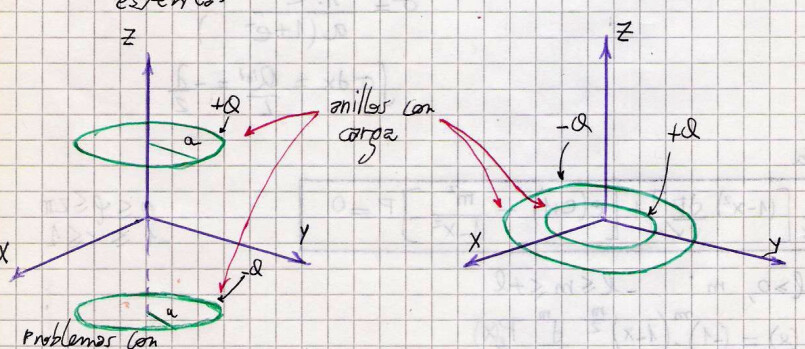
\includegraphics[width=0.5\textwidth]{images/fig_ft1_eje_proble_prolonga.jpg}

Ahora consideraremos la siguiente figura

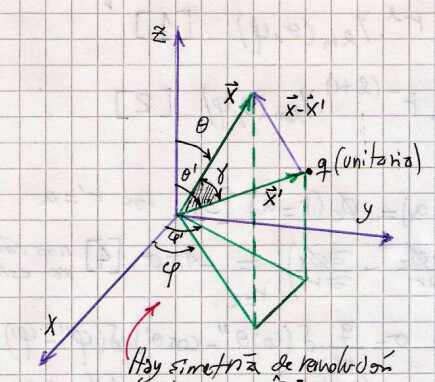
\includegraphics[width=0.5\textwidth]{images/fig_ft1_ejez_separacionEsfericas.jpg}
\\
y la evaluación del potencial 
\[
	\frac{1}{|\vbx - \vbx'|} = \sum_{\ell} \: 
	[ \: A_\ell r^\ell + B_\ell r^{-(\ell +1 )} \: ] \: P_\ell ( \cos \gamma )
\]
Claramente hay simetría de revolución si la carga $q$ se hallase sobre el eje $z$. 
En este caso el problema no puede depender de $\vp$ y ello se ve en que 
$P_\ell ( 1 ) = 1$ para todo $\ell$.

La siguiente figurita explicita lo que sucede
\begin{figure}[bht]
	\begin{center}
	\includegraphics[width=0.7\textwidth]{images/fig_ft1_armesf1.pdf}	 
	\end{center}
	\caption{Figurin}
\end{figure}

Se ve que si $q$ está en $\hat{z}$ entonces la simetría de revolución implica que
$\gamma $ se transforma en el $\theta$ de esféricas.  
Si, además,  $\gamma $ es nulo entonces se tiene simetría de revolución en
torno al eje determinado por la recta que contiene a ambos puntos.

\begin{figure}[tb]
	\begin{center}
	\includegraphics[width=0.2\textwidth]{images/fig_ft1_armesf2.pdf}	 
	\end{center}
	\caption{}
\end{figure} 

Con respecto al inverso de la distancia recíproca resulta
\[
	\frac{1}{|\vb{x}-\vb{x}'|} = \frac{1}{\sqrt{r^2 + {r'}^2  - 2rr'\cos(\gamma)}} \Rightarrow
	\frac{1}{\sqrt{r^2 + {r'}^2  - 2rr'\cos(\theta)}}
\]
donde $|\vb{x}|=r$ y $|\vb{x}'|=r'$. Así
\[
	\left. \frac{1}{|\vb{x}-\vb{x}'|} \right|_{\gamma=0} = \frac{1}{\sqrt{r^2 + r'^2 -2rr'}}=
	\frac{1}{|r-r'|}
\]
Esto define dos zonas \textcircled{1} $r'>r$ y \textcircled{2} $r'<r$.
Serán $\phi_1 = \sum_\ell A_\ell r^\ell$ y $\phi_2 = \sum_\ell B_\ell r^{-(\ell+1)}$.
Entonces, si $r'<r$ será
\[
	\frac{1}{|r-r'|} = \frac{1}{r(1 - r'/r )} = \frac{1}{r} \sum_{\ell=0}^\infty \left(\frac{r'}{r}\right)^\ell = 
	\sum_{\ell=0}^\infty \frac{r'^\ell}{r^{\ell+1}}
\]
en cambio si es $r'>r$
\[
	\frac{1}{|r-r'|} = \frac{1}{r'(1 - r/r' )} = \frac{1}{r'} \sum_{\ell=0}^\infty \left(\frac{r}{r'}\right)^\ell = 
	\sum_{\ell=0}^\infty \frac{r^\ell}{r'^{\ell+1}}
\]
de manera que
\[
	\left. \frac{1}{|\vb{x}-\vb{x}'|} \right|_{\gamma=0} = \sum_{\ell=0}^\infty  \frac{r_<^\ell}{r_>^{\ell+1}}
\]
donde $r_<$ y $r_>$ son el mayor y el menor $r$ para cada región.
Con esta notación se puede escribir una única fórmula.
Además podemos pensar en $1 = P_\ell( 1 ) \forall \ell$ que también es $ 1 = P_\ell(\cos 0 )$, 
lo cual nos lleva a 
\[
	\left. \frac{1}{|\vb{x}-\vb{x}'|} \right|_{\gamma=0} = \sum_{\ell=0}^\infty  \frac{r_<^\ell}{r_>^{\ell+1}}
	P_\ell(\cos 0)
\]
que es la descomposición en polinomios de Legendre del $\phi$ de una carga unitaria
en $\hat{z}$ y evaluado en $\hat{z}$.

Hacemos de esta manera prolongación analítica,
\[
	\frac{1}{|\vb{x}-\vb{x}'|}  = \sum_{\ell=0}^\infty  \frac{r_<^\ell}{r_>^{\ell+1}}
	P_\ell(\cos \gamma)
\]
y decimos que será el $\phi$ de una carga unitaria en cualquier parte
(descompuesto en polinomios de Legendre).
Aquí $\gamma=\gamma(\theta,\varphi)$ de modo que $\cos\gamma$  será una función muy complicada de los ángulos
esféricos, en efecto,
\[
	\cos\gamma = \cos \theta \cos \theta' + \sin \theta \sin \theta' \cos( \vp - \vp').
\]
Se separará el espacio en las dos regiones definidas previamente,
y entonces tendremos
\be
	r < r': \qquad 
	\phi_1(r,\theta,\varphi) = 
	\sum_{\ell=0}^\infty \sum_{m=-\ell}^\ell 
	A_{\ell,m}r^\ell  Y_{\ell,m}(\theta,\varphi)
	\label{phi_1}
\ee
\be
	r > r': \qquad 
	\phi_2(r,\theta,\varphi) = 
	\sum_{\ell=0}^\infty \sum_{m=-\ell}^\ell 
	D_{\ell,m} r^{-(\ell+1)} Y_{\ell,m}(\theta,\varphi)
	\label{phi_2}
\ee

Con estas prescripciones aplicaremos las condiciones de contorno: el potencial será nulo en el infinito,
en la superficie será continuo y no habrá divergencias en el interior de la esfera.

\[
	\phi_1(r=a) = \phi_2(r=a)
\]
\be
	\left( \dpar{\phi_2}{r} - \dpar{\phi_1}{r} \right)_{r=a} = - 4 \pi \sigma
	\label{contorno_2}
\ee
donde esta última $\sigma$ cumple que\footnote{Es una delta de Dirac adecuada para que se cumpla lo que
se tiene que cumplisr}
\[
	\int \sigma dS = q \qquad \sigma = \frac{q}{a^2} \delta(\cos\theta'' - \cos\theta') \delta(\vp''-\vp')
\]

Luego, usando la relación para la $\delta $ anterior se tienen
\[
	\sigma = \frac{q}{a^2} \: Y_{\ell,m}(\theta'',\varphi'') Y_{\ell,m}^*(\theta',\varphi')
\]
y evaluando 
\[
	\phi_1(r'=a) = \phi_2(r'=a)
\]
se tiene $D_{\ell m} = A_{\ell m} a^{2\ell +1}$ puesto que las ecuaciones \eqref{phi_1} y \eqref{phi_2}
son iguales término a término ya que los armónicos independientes son linealmente independientes.

Utilizando la \eqref{contorno_2} con la $\sigma$ definida se llega a que
\[
	\: \sum_{\ell,m} \: 
	\left[ D_{\ell m}(\ell +1) a^{-(\ell + 2)} + A_{\ell m} \ell a^{\ell - 1 } \right] 
	Y_{\ell,m}(\theta,\varphi) =
	\frac{4 \pi q}{a^2} \: \sum_{\ell,m} \: Y_{\ell,m}^*(\theta',\varphi') \: Y_{\ell,m}(\theta,\varphi).
\]
Otra vez usando que son funciones linealmente independientes, se tiene
\[
	\frac{D_{\ell m}^{\ell +1}}{a^{\ell + 2}} + A_{\ell m} \ell a^{\ell - 1 } = 
	\frac{4 \pi q}{a^2} \: Y_{\ell,m}^*(\theta',\varphi')
\]

Ya tenemos los ceoficientes y entonces podemos expresar
el potencial $\phi$ descompuesto en armónicos esféricos como
\[
	\frac{1}{|\vb{x}-\vb{x}'|}  = \sum_{\ell=0}^\infty \sum_{m=-\ell}^\ell \frac{r_<^\ell}{r_>^{\ell+1}}
	\frac{4\pi}{2\ell+1} Y_{\ell,m}(\theta,\varphi) Y_{\ell,m}^*(\theta',\varphi')
\]
que es el potencial de una carga puntual unitaria con armónicos esféricos.
Con esta expresión debiera hacerse más sencilla la integral de Poisson, pero no
tanto porque como sumamos sobre $\ell$ y $m$ la expresión es simétrica por los
índices.

El polinomio $P_\ell$ en función del $\cos\gamma$ se puede escribir utilizando
el {\it teorema de adición} de los armónicos esféricos ha sido usado
\[
	P_\ell(\cos \gamma) = \sum_{m=-\ell}^\ell \frac{4\pi}{2\ell+1} Y_{\ell,m}(\theta,\varphi) 
	Y_{\ell,m}^*(\theta',\varphi')
\]

Ahora, si reemplazamos en la integral de Poisson se tiene
\[
	\phi(\vb{x})= \int_{V'} \rho(\vb{x}')\left[ \sum_{\ell=0}^\infty \sum_{m=-\ell}^\ell 
	\frac{r_<^\ell}{r_>^{\ell+1}}\frac{4\pi}{2\ell+1} Y_{\ell,m}(\theta,\varphi) 
	Y_{\ell,m}^*(\theta',\varphi')\right] dV',
\]
que se puede cosmetizar como
\[
	\phi(\vb{x})= 4\pi \sum_{\ell=0}^\infty \sum_{m=-\ell}^\ell \frac{1}{2\ell+1} \left[
	\int_{V'} \rho(\vb{x}') Y_{\ell,m}^*(\theta',\varphi') {r'}_<^\ell dV' \right] 
	\frac{Y_{\ell,m}(\theta,\varphi) }{r_>^{\ell+1}},
\]
definiéndose el corchete como $q_{\ell m}$ coeficiente multipolar de orden $\ell,m$, así
\[
	\phi(\vb{x})= 4\pi \sum_{\ell=0}^\infty \sum_{m=-\ell}^\ell \frac{q_{\ell m}}{2\ell+1} 
	\frac{Y_{\ell,m}(\theta,\varphi) }{r_>^{\ell+1}},
\]
es el desarrollo multipolar para el potencial $\phi$.

Entonces, definiendo 
\[
	\phi_{\ell m}(\vb{x})= 
	4\pi \frac{q_{\ell m}}{2\ell+1}\frac{Y_{\ell,m}(\theta,\varphi) }{r_>^{\ell+1}}
\]
se tiene para el campo eléctrico
\[
	\vb{E}(\vb{x}) = - \Nabla \phi(\vb{x})= 
	-\Nabla \sum_{\ell,m} \phi_{\ell m}(\vb{x}) =
	\sum_{\ell,m} \vb{E}_{\ell m}(\vb{x})
\]
que es una suma de campos multipolares
\[
	\vb{E}_{\ell m}(\vb{x}) = - \Nabla \phi_{\ell m}(\vb{x}).
\]

\subsection{Relación de los multipolos esféricos y los cartesianos}

El operador gradiente en coordenadas esféricas es Apéndice XXX.
Entonces
\[
	E_r^{\ell m} = \frac{4\pi(\ell+1)}{ 2\ell+1 } 
	\frac{Y_{\ell,m}(\theta,\varphi) }{r^{\ell+2}} \: q_{\ell m}
\]
\[
	E_\theta^{\ell m} = \frac{-2\pi}{2\ell+1} \frac{1}{r^{\ell+2}}
	\dpar{Y_{\ell,m}(\theta,\varphi) }{\theta} \: q_{\ell m}
\]
\[
	E_\vp^{\ell m} = \frac{-4\pi}{2\ell+1} \frac{ i m}{r^{\ell+2}\sin\theta} 
	Y_{\ell,m}(\theta,\varphi) \: q_{\ell m}
\]
De aquí, reemplazando sale la relación entre desarrollos
\[
	q_{00} = \frac{q}{\sqrt{4\pi}} \qquad \qquad Y_{00} = Y_{00}^* = \frac{1}{\sqrt{4\pi}}
\]
\[
	\ell = 1 \qquad 
	\begin{cases}
	q_{1,1} = - \sqrt{\frac{3}{4\pi}}( p_x -i p_y ) \\
	\\
	 q_{1,-1} = \sqrt{\frac{3}{4\pi}}( p_x + i p_y ) \\
	 \\
	 q_{1,0} = \sqrt{\frac{3}{4\pi}} \: p_z
	\end{cases}
	\qquad 
	Y_{11} = -\sqrt{\frac{3}{8\pi}}  \sin\theta \: \euler^{i\vp}
\]
\[
	(-1)^m q_{\ell m}^* = q_{\ell,-m}
\]
\[
	\begin{cases}
	q_{20} = \frac{1}{2} \sqrt{\frac{5}{4\pi}} Q_{33} \\
	\\
	 q_{21} = - \frac{1}{3} \sqrt{\frac{15}{2\pi}}( Q_{13} -i Q_{23} ) \\
	 \\
	 q_{22} = - \frac{1}{12} \sqrt{\frac{15}{2\pi}}( Q_{11} - 2 i Q_{12} - Q_{22} )	 
	\end{cases}
	\quad 
	Y_{20} = \sqrt{\frac{5}{4\pi}}\left(  \frac{3}{2} \cos^2\theta - \frac{1}{2} \right)	
\]
donde en estas últimas expresiones los índices numéricos representan las
coordenadas de acuerdo con $1,2,3 \equiv x,y,z$.

% =================================================================================================
\section{Separación de variables en cilíndricas}
% =================================================================================================

Se propone
\[
	\phi(\rho,\phi,z) = R(\rho) Q(\phi) Z(z)
\]
de modo que el laplaciano en cilíndricas (ver Apéndice XXX) conduce a
\[
	\frac{1}{R} \dtot[2]{R}{\rho} + \frac{1}{R\rho} \dtot{R}{\rho} + \frac{1}{Q\rho^2} \dtot[2]{Q}{\phi} 
				+ \frac{1}{Z} \dtot[2]{Z}{z} = 0.
\]
Entonces
\[
	\frac{1}{Z} \dtot[2]{Z}{z} = k^2
\]
donde la naturaleza de $k$ dependerá también de las condiciones de contorno
del problema.
Entonces podemos escribir
\[
	\frac{\rho^2}{R} \dtot[2]{R}{\rho} + 
	\frac{\rho}{R} \dtot{R}{\rho} + 
	\frac{1}{Q} \dtot[2]{Q}{\phi} 
	+ \rho^2 k^2 = 0.
\]
y hacemos
\[
	\frac{1}{Q} \dtot[2]{Q}{\phi} = -\nu^2
\]
donde la constante se toma negativa por la condición de que $Q$ sea periódica
en $2\pi$.


Donde los primeros dos términos conducen a la ecuación de Bessel, el tercero es igual a $-\nu^2$ y el
cuarto a $k^2$. Sacamos
\[
	Z = \euler^{\pm kz}
\]
\[
	Q = \euler^{\pm i \nu \phi}
\]
donde si $0\leq \phi \leq 2\pi$ entonces $\nu \in \mathbb{Z}$. Si en cambio la variable $\phi$ no corre 
entre $0$ a $2\pi$ se dará que $\nu \notin \mathbb{Z}$.

\begin{center}
	\begin{tabular}{|c|c|}
	\hline
	$ \nu \in \mathbb{Z} $ & $ \nu \notin \mathbb{Z}  $ \\
	\hline
	$J_\nu(k\rho)$ & $J_\nu(k\rho)$ \\
	$J_{-\nu}(k\rho)$ & $N_\nu(k\rho)$ \\
	\hline
	\end{tabular} 
\end{center}
donde 
\[
	N_\nu(k\rho) \equiv \frac{ J_\nu(k\rho) \cos(\nu\pi) - J_{-\nu}(k\rho)}{\sin(\nu\pi)}
\]
siendo $J_\nu(k\rho)$ la función de Bessel de primera especie, $N_\nu(k\rho)$ la función de Bessel de segunda 
especie (Neumann).
$N_\nu(k\rho)$ tiene problemas en el origen de modo que no sirve si el dominio incluye al eje $\hat{z}$, en 
cambio $J_\nu(k\rho)$ tiene problemas en $\rho\to \infty$.

También se suelen definir
\[
	H^{(1)}_\nu(k\rho) = J_\nu(k\rho) + i N_\nu(k\rho)
\]
\[
	H^{(2)}_\nu(k\rho) = J_\nu(k\rho) - i N_\nu(k\rho)
\]
que son las funciones de Bessel de tercera especie o bien Hankel de primera y segunda especie respectivamente.

\subsubsection{Cambio de signo de la constante de separación}

\[
	... + \underbrace{\frac{1}{Z} \dtot[2]{Z}{z}}_{-k^2} =  0
\]
entonces nos lleva a
\[
	Z = \euler^{\pm i k z} \qquad \qquad Q = \euler^{\pm i \nu \phi}
\]
y entonces a las funciones de Bessel modificadas
\[
	I_\nu(k\rho) = i^{-\nu} J_\nu(k\rho)
\]
\[
	K_\nu(k\rho) = \frac{\pi}{2}i^{\nu+1} H_\nu^{(1)}(k\rho),
\]
donde son respectivamente las de primera y segunda especie y vemos que tienen argumento imaginario.
Las $I_\nu(k\rho)$ tendrán problemas en $\rho\to\infty$ y $K_\nu(k\rho)$ problemas en $\rho=0$ (en el eje 
$\hat{z}$).
Si atravesamos densidades de carga en $\hat{z}$ entonces usamos Bessel
\[
	Z = \euler^{\pm k z} \quad \Rightarrow \quad J_\nu^{(1)}(k\rho) ; N_\nu^{(2)}(k\rho)
\]
pero bajo condiciones periódicas en $\hat{z}$ se usan Bessel modificadas
\[
	Z = \euler^{ \pm i k z} \quad \Rightarrow \quad I_\nu^{(1)}(k\rho) ; K_\nu^{(2)}(k\rho)
\]
y esto último se da por ejemplo en tapas del cilindro.
La función de Bessel de primera especie se puede expresar como serie según
\[
	J_\nu^{(1)}(k\rho) = \left(\frac{x}{2}\right)^\nu \sum_{j=0}^\infty \frac{(-1)^j}{j!\Gamma(j+\nu +1)} 
		\left(\frac{x}{2}\right)^{2j}
\]

Las funciones de Bessel tienen infinitos ceros,
\[
	J_\nu(x_{\nu n}) = 0 \qquad \mathrm{con} \; n\in\mathbb{N}, \nu \quad \mathrm{fijo} 
\]
siendo $x_{\nu n}$ un cero de $J_\nu$. Así
\[
	\sqrt{\rho} J_\nu(x_{\nu n} \rho/a) 
\]
con $\nu \geq 0$ fijo es un conjunto ortonormal completo en $0 \leq \rho \leq a$ siendo $a$ el radio del 
cilindro.
\[
	f(\rho) = \sum_{n=1}^{\infty}  A_{x_{\nu n}} J_{\nu}( x_{\nu n} \rho/a )
\]
con $0 \leq \rho \leq a$. Así $f(\rho=a)=0$,
\[
	A_{\nu n} = \frac{2}{a^2 J_{\nu +1}^2 (x_{\nu n})} \int_0^a \rho f(\rho) J_\nu (x_{\nu n} \rho/a) 
	d\rho
\]
la ortogonalidad
\[
	\int_0^a \rho  J_\nu (x_{\nu n'} \rho/a)  J_\nu (x_{\nu n} \rho/a)  d\rho = 
	\frac{a^2}{2}[J_{\nu+1}(x_{\nu n})]^2 \delta_{nn'}.
\]

Para $k$ sea $\phi(\rho=a)=0$ entonces 
\[
	J_\nu(ka) = 0 \Rightarrow ka=x_{\nu n} \Rightarrow J_\nu (x_{\nu n} \rho/a)
\]
y $k=\frac{x_{\nu n}}{a}$ si $0\leq \rho \leq a$ y si está acotado en $\rho$ entonces es discreto y se
suma $\sum_{n=1}^\infty$ y $\nu\to m \in \mathbb{Z}$ si $0 \leq \phi \leq 2\pi$ y si no está acotado en
$\rho$ entonces usamos 
\[
	\int_0^\infty dk
\]
y la completitud
\[
	\int_0^\infty x J_\nu(kx) J_\nu(k'x) dx = \frac{1}{k} \delta (k-k')
\]
y $k$ en general será función de $n\in \mathbb{N}$ por condición periódica en tapas (en $\hat{z}$) o en
cilindros (en $\hat{\rho}$).
\[
	\phi(\rho,\phi,z) = \sum_{\nu=0}^\infty \sum_{n=1}^\infty
	[A_{\nu k}\begin{cases} J_\nu(k\rho)  \\ I_\nu(k\rho) \end{cases} + 
	B_{\nu k} \begin{cases} N_\nu(k\rho)  \\ K_\nu(k\rho) \end{cases} ]
	[C_k \begin{cases} \euler^{\pm kz} \\ \euler^{\pm ikz} \end{cases}]
	[D_{k\nu} \euler^{\pm i \nu \phi}]
\]
donde $k=k(n)$ y usamos $\sin(kz)+\cos(kz)$ si hay discretización.



% \bibliographystyle{CBFT-apa-good}	% (uses file "apa-good.bst")
% \bibliography{CBFT.Referencias} % La base de datos bibliográfica

\end{document}
